\documentclass{beamer}
\usepackage{booktabs}
\usepackage{graphicx}
\usepackage{amsmath}
\usepackage{array}
\usetheme{default}
\setbeamertemplate{navigation symbols}{}
\setbeamertemplate{footline}{\hfill\insertframenumber/\inserttotalframenumber\hspace{1.5em}}

\title{Robust Constraint Learning: Research Update}
\subtitle{Reactor tested against the ODE; gastric folds $+$ full in}
\date{8 September 2026}

\begin{document}

% ===========================================================================
\begin{frame}{Since the last update (28 Aug)}
    \scriptsize
    \begin{itemize}
        \item \textbf{Compared our implementation of C-MICL against Ovalle et al.'s own code}
              \begin{itemize}\scriptsize
                  \item MIP constrains (residual model) $u(x)\ge0$, fixed $32{\times}32$ width net.
                  \item \textbf{Under their own $c$ draw}
                  \item Still not replicating their results (we get 0.27 feasibility vs their 0.9), but we have
                        some differences in implementation: model determined by CV to allow comparison
                        with other methods, theirs' fixed, slightly smaller sample size to allow
                        subsampling (worst-case results).
                  \item They have different versions, unclear which is used in the paper.
                        Try to run exactly as they do / ask them?
              \end{itemize}
        \item \textbf{For our results next: Reactor cost vector: ones $\to$ balanced} ($1/\text{span}_i$).
              So each decision variable contributes roughly equally to objective. Note this differs from Ovalle et al.
        \item \textbf{Two parameters to tune: Reactor $\rho$ columns re-derived} on the balanced instance,
              $\rho\,1$--$6$ walked whole: CP $\{1,2\}$, wrapper $\{3,4\}$ ---
              each brackets \emph{its own} transition.
    \end{itemize}
\end{frame}

% ===========================================================================
% run_dial_sweep.py --problem reactor (rho 1-6, --refresh --search grid, 09-04)
% run_dial_test.py --problem reactor (09-07)
\begin{frame}{Reactor: tuned on the proxy, tested on the ODE}
    \scriptsize
    Folds $=10$; full $=$ one refit. Min = lower objective better.
    Solve time is the mean master solve at the row's dial in the \emph{tuning}
    run (train $+$ build $+$ solve; for CP the whole cut loop) --- a runtime,
    not part of the cost.
    \textbf{Bold} $=$ best cost among the rows that reach $0.9$.
    {\scriptsize\setlength{\tabcolsep}{3pt}
    \begin{tabular}{llccc|c|c}
        \toprule
        & & \multicolumn{3}{c|}{feasibility} & cost (min) & solve \\
        \cmidrule(lr){3-5}\cmidrule(lr){6-6}\cmidrule(lr){7-7}
        method & dial$^\ast$ & proxy & \textbf{ODE} fold & \textbf{ODE} full
               & ODE folds & master (s) \\
        \midrule
        nominal            & --           & 0.00 & 0.00 & 0.00
                           & $5.506\pm0.07$ & 0.5 \\
        CP $\rho{=}2$      & $\tau=0.3$   & 0.90 & 1.00 & 1.00
                           & $\mathbf{5.816}\pm0.04$ & 1.8 \\
        wrapper $\rho{=}4$ & $\alpha=0$   & 0.90 & 1.00 & 1.00
                           & $5.885\pm0.07$ & 2.6 \\
        RHS margin         & $m=4.0$      & 1.00 & 1.00 & 1.00
                           & $6.043\pm0.07$ & 2.2 \\
        C-MICL prot.       & $\alpha=0.1$ & --   & 0.20 & 1.00
                           & $5.666\pm0.11$ & 6.3 \\
        \midrule
        \multicolumn{7}{l}{\emph{ceiling}: no dial$^\ast$; most-feasible cell} \\
        CP $\rho{=}1$      & $\tau=0.1$   & 0.30 & 0.70 & 1.00 & $5.706\pm0.03$ & 1.2 \\
        wrapper $\rho{=}3$ & $\alpha=0$   & 0.40 & 0.90 & 1.00 & $5.788\pm0.05$ & 2.3 \\
        wrapper $\rho{=}2$ & $\alpha=0$   & 0.10 & 0.70 & 0.00 & $5.701\pm0.05$ & 1.6 \\
        C-MICL             & $\alpha=0.3$ & 0.10 & 0.10 & 1.00 & $5.638\pm0.08$ & 5.8 \\
        \bottomrule
    \end{tabular}}
    \begin{itemize}\scriptsize
        \item \textbf{At equal tuned feasibility (0.9), CP is cheapest}:
              $5.816 <$ wrapper $5.885 <$ margin $6.043$. Nominal cheaper but infeasible.
        \item C-MICL infeasible at its own asserted $\alpha$.
    \end{itemize}
\end{frame}

% ===========================================================================
\begin{frame}{Gastric: sweep complete, folds $+$ full tested}
    \scriptsize
    Judge $=$ GT ensemble on all 416 arms; OS is a \textbf{max}. Folds $=145$
    decisions over 4 temporal folds; full $=$ the 96 held-out arms. Key result is held-out 96.
    \textbf{Bold} $=$ best OS among the rows at feas $\ge0.9$ in that column.
    \textbf{Feas and OS are over each method's \emph{own} solved arms} ---
    different denominators per row, so read them beside solved. The common-cohort
    (samestore) numbers come with the subsample phase.
    {\scriptsize\setlength{\tabcolsep}{3pt}
    \begin{tabular}{llcc|cc|cc}
        \toprule
        & & \multicolumn{2}{c|}{tuned} & \multicolumn{2}{c|}{folds}
          & \multicolumn{2}{c}{held-out 96} \\
        \cmidrule(lr){3-4}\cmidrule(lr){5-6}\cmidrule(lr){7-8}
        method & dial$^\ast$ & feas & solved & feas & OS & feas & OS \\
        \midrule
        nominal              & --           & 0.891 & 0.951 & 0.925 & \textbf{11.30} & 0.957 & \textbf{12.33} \\
        RHS margin           & $m=0.2$      & 0.931 & 0.922 & 0.951 & 11.01 & 0.978 & 12.27 \\
        wrapper $\rho{=}0.5$ & $\alpha=0.2$ & 0.941 & 0.679 & 0.961 & 10.97 & 0.988 & 12.15 \\
        wrapper $\rho{=}1$   & $\alpha=0.6$ & 0.903 & 0.643 & 0.971 & 10.97 & 0.887 & 12.36 \\
        CP $\rho{=}0.5$      & $\tau=0.03$  & 0.974 & 0.821 & 0.987 & 10.86 & 0.957 & 12.26 \\
        CP $\rho{=}1$        & $\tau=0.1$   & 0.938 & 0.870 & 0.936 & 10.07 & 0.978 & 12.24 \\
        C-MICL               & $\alpha=0.6$ & 0.919 & 0.893 & 0.931 & 10.03 & 0.944 & 11.71 \\
        C-MICL prot.         & $\alpha=0.1$ & --    & 0.081 & 1.000 & 9.34  & 0.895 & 10.92 \\
        \bottomrule
    \end{tabular}}
    \begin{itemize}\scriptsize
        \item \textbf{Nominal is already at target} in held-out 96. 
            Should we increase the feasibility target for this instance to $>$ 0.957?
        \item \textbf{C-MICL at its asserted $\alpha{=}0.1$}: feasibility
              $1.000$ / $0.895$, but on $12/145$ and $19/96$ contexts --- it
              declines for $\sim$90\% of patients, one fold entirely.
        \item \textbf{Subsample: 3 of 10 draws still running.} Will give worst-case.
    \end{itemize}
\end{frame}

% ===========================================================================
% fig regenerated 2026-09-08 from the completed gastric curve (plot_dial_sweep.py
% --problem gastric --suffix _incoh_s42 --xlim auto --compact)
\begin{frame}{Gastric: the tuning frontier (all series, widened grids)}
    \begin{center}
    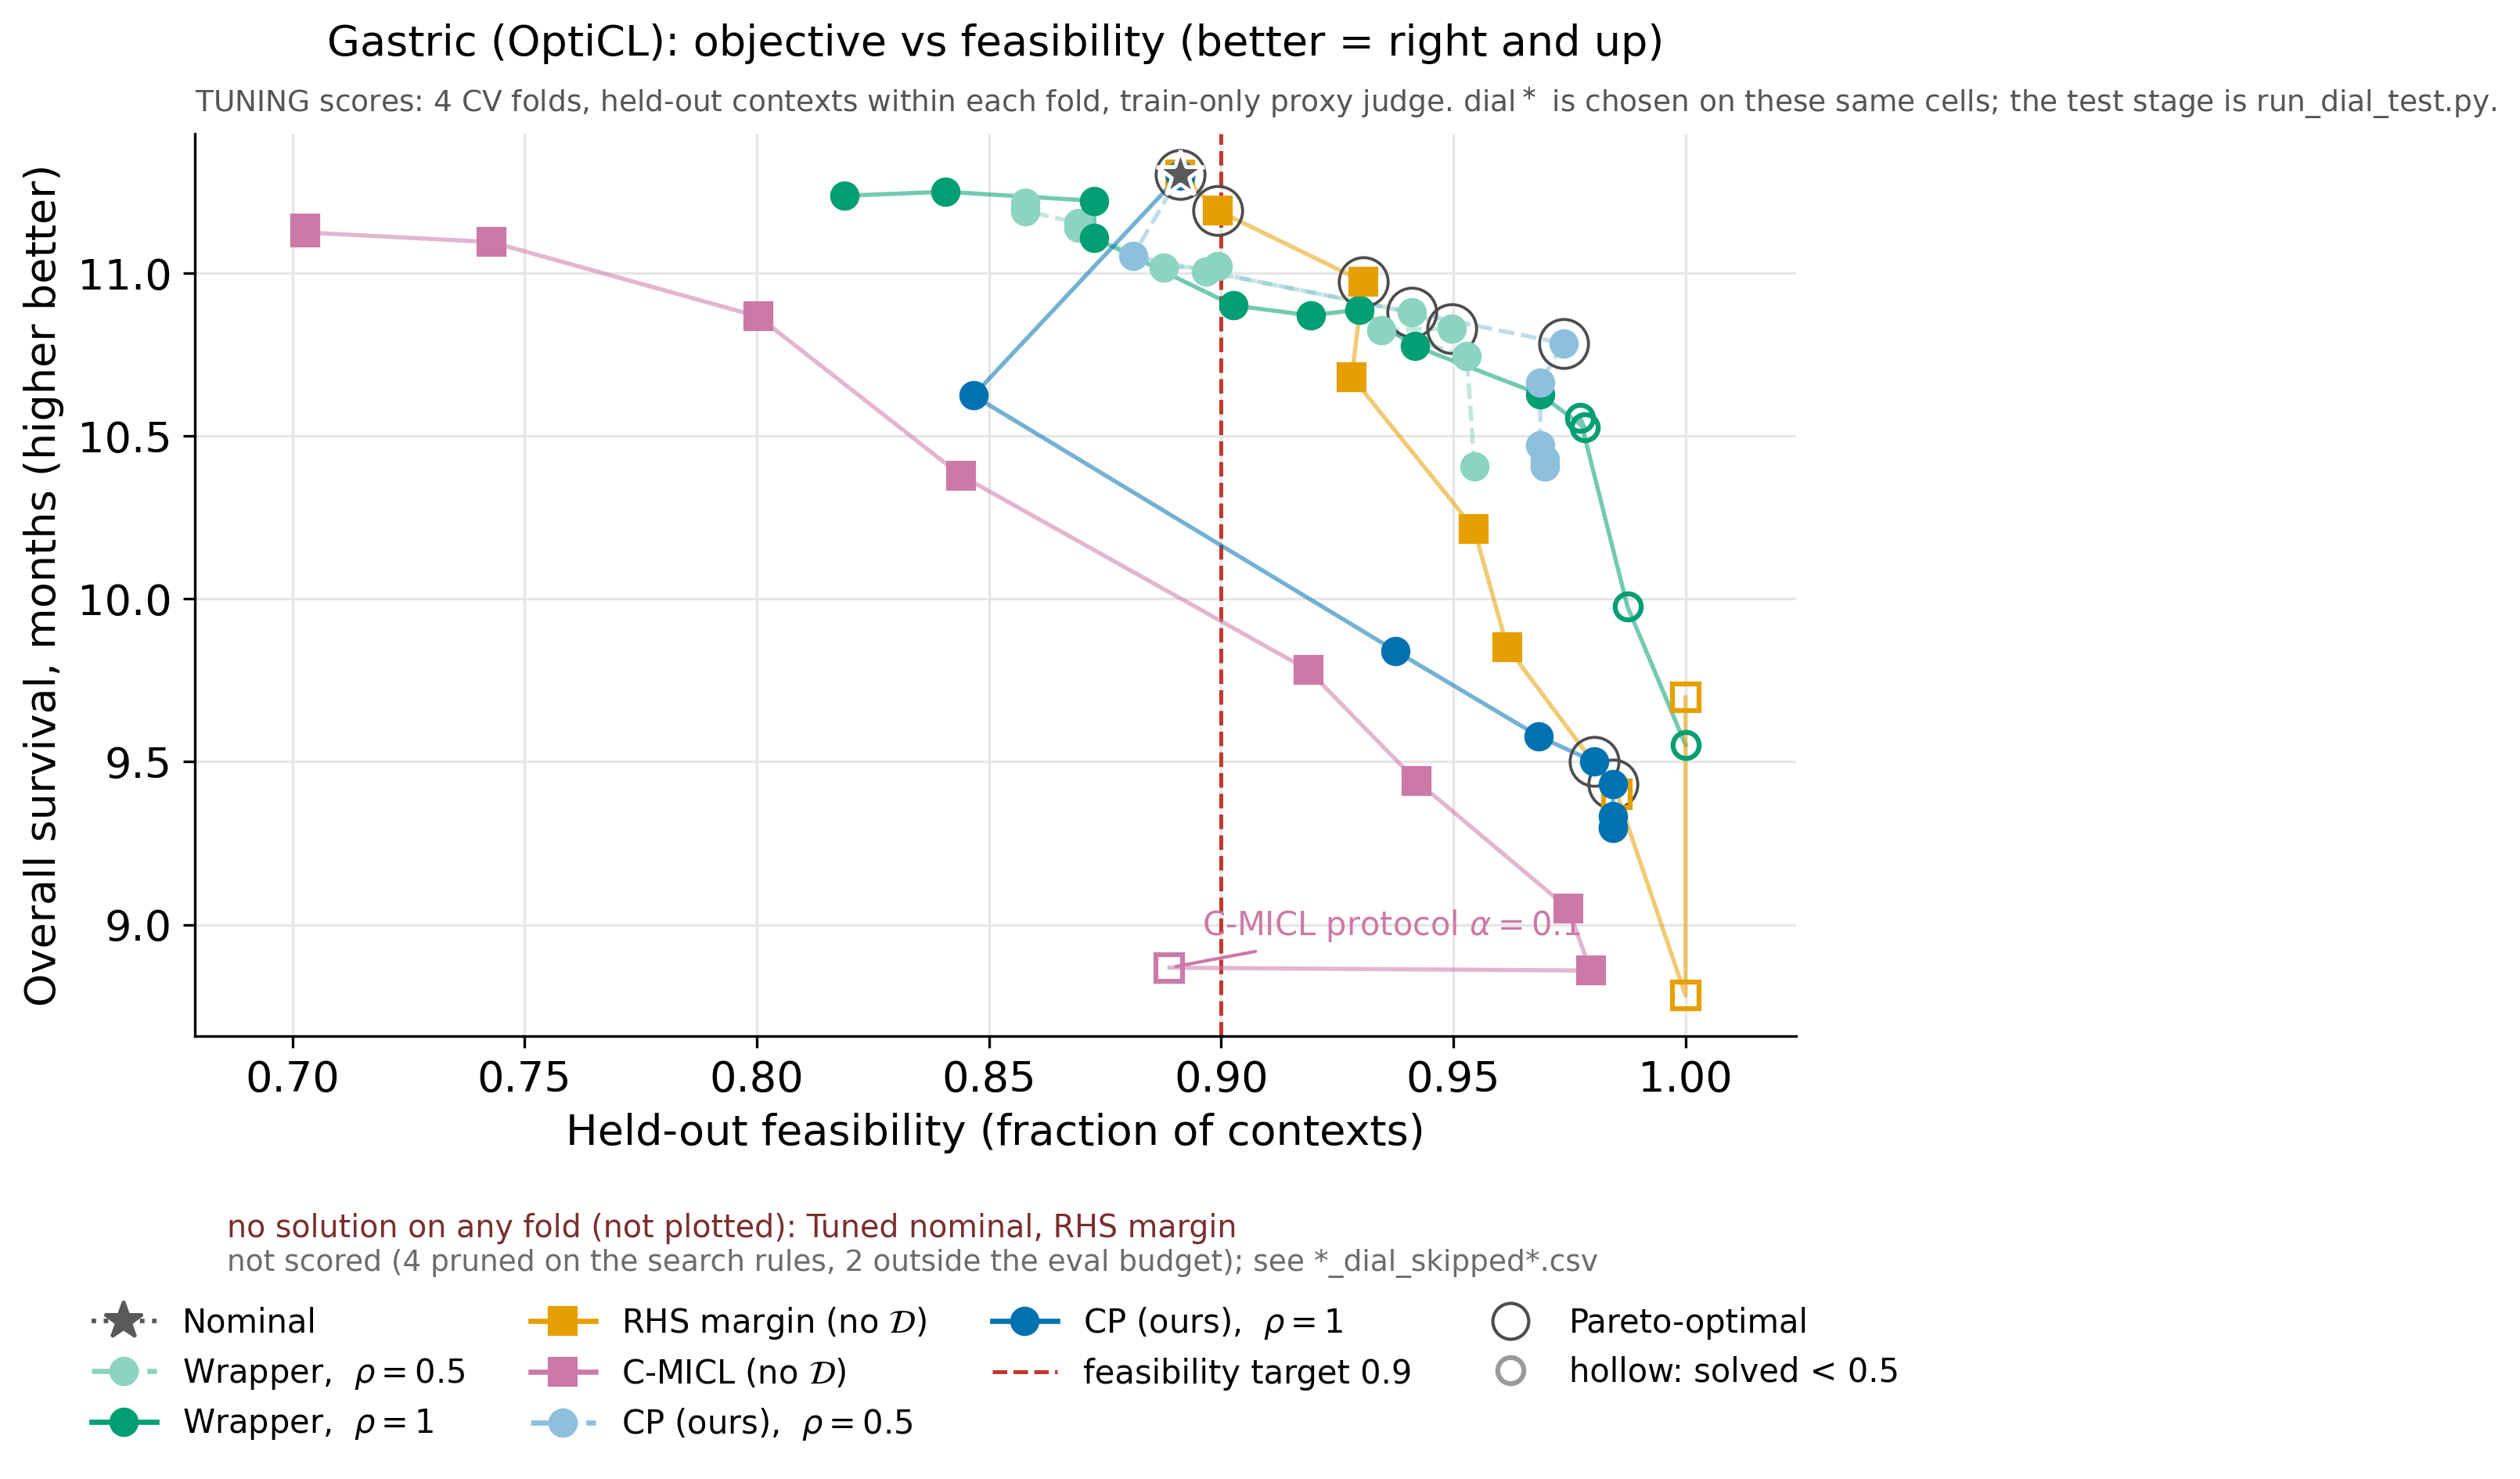
\includegraphics[width=\linewidth,height=0.6\textheight,keepaspectratio]{../results/figures/fig_dial_frontier_gastric_incoh_s42_slide.png}
    \end{center}
    \vspace{-0.5em}
    \begin{itemize}\scriptsize
        \item \textbf{TUNING scores} --- dial$^\ast$ is chosen on these same
              cells; tested numbers are the previous frame.
        \item \textbf{C-MICL (pink) is dominated across its whole grid}: at
              matched feasibility it gives up $1$--$2$ months of OS, and its
              protocol $\alpha{=}0.1$ sits at the bottom edge.
        \item \textbf{Hollow $=$ solved $<0.5$; read it before reading height.}
              The wrapper's high-feasibility end solves $64$--$68\%$ of contexts
              against CP's $82$--$87\%$.
    \end{itemize}
\end{frame}

% ===========================================================================
\begin{frame}{Next steps}
    \footnotesize
    \begin{enumerate}
        \item \textbf{Key Questions}
            \begin{itemize}\scriptsize
                  \item Try to replicate Ovalle et al.'s results with their code? (We have a few differences in implementation.)
                  \item Should we increase the feasibility target for gastric to $>$ 0.957?
            \end{itemize}
        \item \textbf{Screen the epigraph objective}
              \begin{itemize}\scriptsize
                  \item CP at the new dial$^\ast$ ($\tau=0.03$ / $0.1$); epigraph
                        on; subsample; CRN-paired against the arm on disk.
                  \item Prize $0.23$ realized-OS tail (nominal worst-of-10 $11.14$
                        vs CP $10.90$) against a draw sd of $0.55$.
                  \item dial$^\ast$ tuned with the epigraph off $\Rightarrow$ a
                        lower bound; full sweep only if it moves.
              \end{itemize}
        \item \textbf{Screen the convex hull (gastric)}
        \item \textbf{WFP food basket.}
              \begin{itemize}\scriptsize
                  \item Shared benchmark of OptiCL and C-MICL --- omitting it reads
                        as selection.
                  \item Palatability label continuous ($6002\times13$) $\Rightarrow$
                        enters the regression framework unchanged.
                  \item \emph{One} learned constraint; nutrients known linear ---
                        gastric stays the multi-constraint instance.
                  \item Open: diet reduction vs.\ full supply chain.
              \end{itemize}
        \item \textbf{Write paper.}
              \begin{itemize}\scriptsize
                  \item CP / RHS margin generalize to multiple constraints, keeping
                        feasibility.
                  \item CP best worst-case feasibility; cut loop is offline.
                  \item CP cheapest at equal feasibility on the reactor's ODE.
                  \item Open: formally extend C-MICL to multiple constraints?
              \end{itemize}
    \end{enumerate}
\end{frame}

\end{document}
